\documentclass[multi,tikz]{standalone}
\usepackage{tikz}
\usepackage{pgfplots}
\pgfplotsset{compat=1.18}

\usetikzlibrary{decorations.pathmorphing}
\usetikzlibrary{decorations.pathreplacing}
\usetikzlibrary{calc,intersections}

\usepackage{pgfplots}
\usepackage{pgfplotstable}
\pgfplotsset{compat=1.18}
\usepgfplotslibrary{fillbetween}
\usepackage{csvsimple}


% LIGHTCONES
\newcommand{\lightconecurved}[5]{% x0=#1, t0=#2, length L=#3 % interior or exterior \pm
	\begin{scope}
		% 1. Inputs
		\pgfmathsetmacro{\xzero}{#1}
		\pgfmathsetmacro{\tzero}{#2}
		\pgfmathsetmacro{\raylen}{#3}
		\pgfmathsetmacro{\region}{#4}
		\pgfmathsetmacro{\rs}{#5}
		
		% 2. Slopes
		\pgfmathsetmacro{\sqrtterm}{sqrt(\rs/\xzero)}
		\pgfmathsetmacro{\den}{1 - \rs/\xzero}
		\pgfmathsetmacro{\mplus}{(\sqrtterm + 1)/(\den)}
		\pgfmathsetmacro{\mminus}{(\sqrtterm - 1)/(\den)}
		
		% 3. Normalization of length of light cone branches
		% Right branch (Positive x direction)
		\pgfmathsetmacro{\drR}{\raylen / sqrt((\mplus)^2 + 1)}
		\pgfmathsetmacro{\xfinr}{\xzero + \region*\drR}
		\pgfmathsetmacro{\tfinr}{\tzero + \region*\mplus * \drR}
		
		% Left branch (Negative x direction)
		\pgfmathsetmacro{\drL}{\raylen / sqrt((\mminus)^2 + 1)}
		\pgfmathsetmacro{\xfinl}{\xzero - \drL}
		\pgfmathsetmacro{\tfinl}{\tzero + \mminus * (-\drL)} % slope * negative change
		
		% 4. "Bake" values to avoid scope errors
		\edef\tempdraw{%
			\noexpand\draw[thick, red] (axis cs:\xzero,\tzero) -- (axis cs:\xfinr,\tfinr);
			\noexpand\draw[thick, red] (axis cs:\xzero,\tzero) -- (axis cs:\xfinl,\tfinl);
			\noexpand\fill[yellow, opacity=0.6] (axis cs:\xzero,\tzero) -- (axis cs:\xfinr,\tfinr) -- (axis cs:\xfinl,\tfinl) -- cycle;
		}
		\tempdraw
	\end{scope}
}

\begin{document}

%
%%
%%% Figure 1 %%%
%%
%
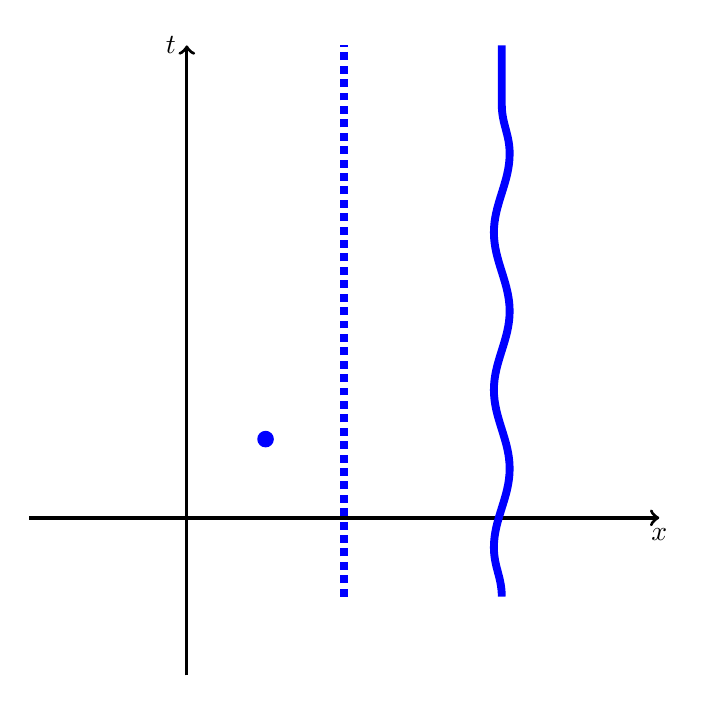
\begin{tikzpicture}
%[scale=0.75,>=latex]

% Draw the time axis (t-axis)
\draw[very thick,->] (0,-2) -- (0,6) node[left] {$t$};

% Draw the space axis (x-axis)
\draw[very thick,->] (-2,0) -- (6,0) node[below] {$x$};

% An event
\fill[blue] (1,1) circle[radius=3pt];

% A series of events
\draw[blue, line width=1mm, dotted] (2,-1) -- (2,6);

% A worldline of a particle moving left and right
\draw[blue, line width=1mm, decorate, decoration={snake, amplitude=1mm, segment length=20mm}] (4,-1) -- (4,6);		
\end{tikzpicture}



%
%%
%%% Figure 2 %%%
%%
%
\begin{tikzpicture}
    %[scale=0.75,>=latex]
% Draw the time axis (t-axis)
\draw[very thick,->] (0,-2) -- (0,6) node[left] {$t$};

% Draw the space axis (x-axis)
\draw[very thick,->] (-2,0) -- (6,0) node[below] {$x$};

\fill[black] (1,0) circle[radius=3pt];
\fill[black] (3,0) circle[radius=3pt];

\fill[black] (0.5,2) circle[radius=3pt];
\fill[black] (4,2) circle[radius=3pt];
\draw[thin,-] (-2,2) -- (6,2);

\fill[black] (2,4) circle[radius=3pt];
\fill[black] (3,4) circle[radius=3pt];
\draw[thin,-] (-2,4) -- (6,4);

\end{tikzpicture}

%
%%
%%% Figure 2.5 %%%
%%
%
\begin{tikzpicture}[scale=0.75,>=latex]
	
	% Draw the time axis (t-axis)
	\draw[very thick,->] (0,-2) -- (0,6) node[left] {$t$};
	
	
	% Draw the space axis (x-axis)
	\draw[very thick,->] (-2,0) -- (6,0) node[below] {$x, \textcolor{blue}{x'}$};
	
	% Draw first mover
	\draw[very thick,->, blue] (0,0) -- (1.5,6) node[left] {$t'$};
	
	
\end{tikzpicture}

%
%%
%%% Figure 3 %%%
%%
%
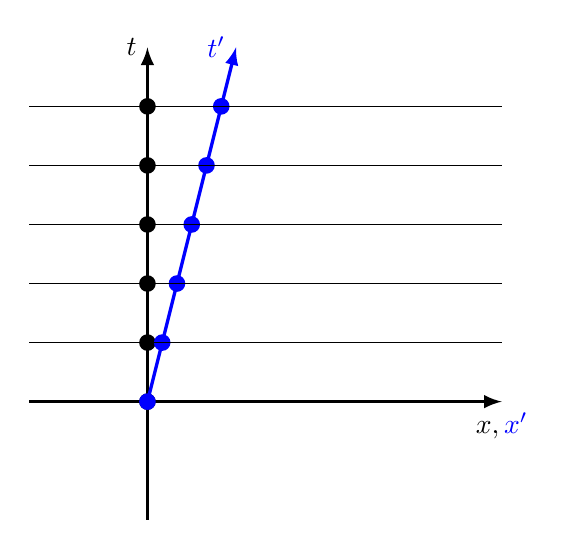
\begin{tikzpicture}[scale=0.75,>=latex]

% Draw the time axis (t-axis)
\draw[very thick,->] (0,-2) -- (0,6) node[left] {$t$};

% Add equally spaced black dots along the t-axis
\foreach \y in {0,1,2,3,4,5}
\fill[black] (0,\y) circle[radius=4pt];

% Draw the space axis (x-axis)
\draw[very thick,->] (-2,0) -- (6,0) node[below] {$x, \textcolor{blue}{x'}$};

% Draw first mover
\draw[very thick,->, blue] (0,0) -- (1.5,6) node[left] {$t'$};

% Add equally spaced blue dots along the t' axis to represent the proper time of the moving observer 
\foreach \y in {0,1,2,3,4,5} \fill[blue] (0.25*\y,\y) circle[radius=4pt];

% Simultaneous lines
\foreach \y in {1,2,3,4,5}
\draw[thin,-,black] (-2,\y) -- (6,\y);

\end{tikzpicture}

%
%%
%%% Figure 4 %%%
%%
%

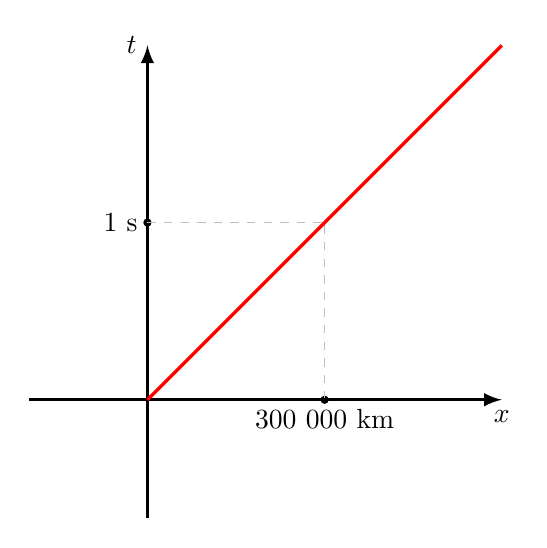
\begin{tikzpicture}[scale=0.75,>=latex]
	
	% Draw the time axis (t-axis)
	\draw[very thick,->] (0,-2) -- (0,6) node[left] {$t$};
	
	\fill[black] (0,3) circle[radius=2pt] node[left] {1 s};
	\fill[black] (3,0) circle[radius=2pt] node[below] {300 000 km};
	\draw[dashed,gray!50] (0,3) -- (3,3);
	\draw[dashed,gray!50] (3,0) -- (3,3);
	
	% Draw the space axis (x-axis)
	\draw[very thick,->] (-2,0) -- (6,0) node[below] {$x$};
	
	% Draw light
	\draw[very thick,-, red] (0,0) -- (6,6) node[left] {$ $};

\end{tikzpicture}

%
%%
%%% Figure 5 %%%
%%
%


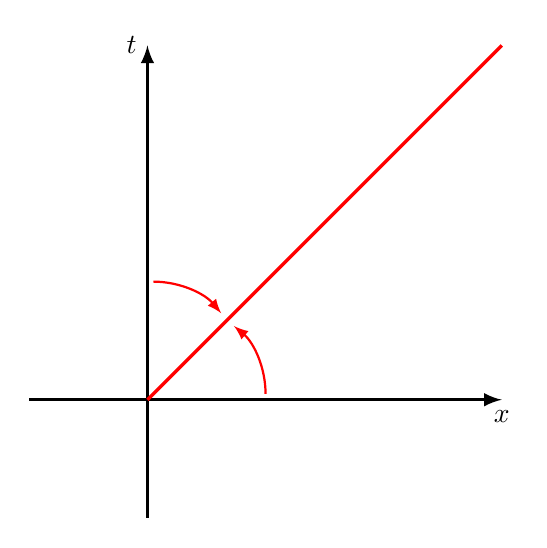
\begin{tikzpicture}[scale=0.75,>=latex]
	
	% Draw the time axis (t-axis)
	\draw[very thick,->] (0,-2) -- (0,6) node[left] {$t$};
	%\draw[->, thick, red] (0.1,2) arc[start angle=120, end angle=55, radius=1.5cm];
	\draw[->, thick, red] (0.1,2) arc[start angle=90, end angle=40, radius=1.5cm];
	\draw[->, thick, red] (2,0.1) arc[start angle=0, end angle=50, radius=1.5cm];
	
	% Draw the space axis (x-axis)
	\draw[very thick,->] (-2,0) -- (6,0) node[below] {$x$};
	
	% Draw light
	\draw[very thick,-, red] (0,0) -- (6,6) node[left] {$ $};
	
\end{tikzpicture}


%
%%
%%% Figure 6 %%%
%%
%
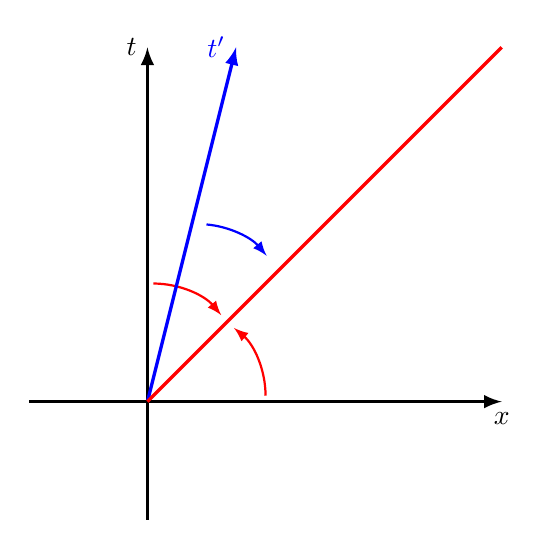
\begin{tikzpicture}[scale=0.75,>=latex]
	
	% Draw the time axis (t-axis)
	\draw[very thick,->] (0,-2) -- (0,6) node[left] {$t$};
	%\draw[->, thick, red] (0.1,2) arc[start angle=120, end angle=55, radius=1.5cm];
	\draw[->, thick, red] (0.1,2) arc[start angle=90, end angle=40, radius=1.5cm];
	\draw[->, thick, red] (2,0.1) arc[start angle=0, end angle=50, radius=1.5cm];

	% Draw first mover
	\draw[very thick,->, blue] (0,0) -- (1.5,6) node[left] {$t'$};
	%\draw[very thick,->, blue] (0,0) -- (6,1.5) node[below] {$x'$};
	
	%\draw[->, thick, blue] (3,1) arc[start angle=0, end angle=45, radius=1.5cm];
	\draw[->, thick, blue] (1,3) arc[start angle=85, end angle=40, radius=1.5cm];
	
	% Draw the space axis (x-axis)
	\draw[very thick,->] (-2,0) -- (6,0) node[below] {$x$};
	
	% Draw light
	\draw[very thick,-, red] (0,0) -- (6,6) node[left] {$ $};
\end{tikzpicture}

%
%%
%%% Figure 7 %%%
%%
%
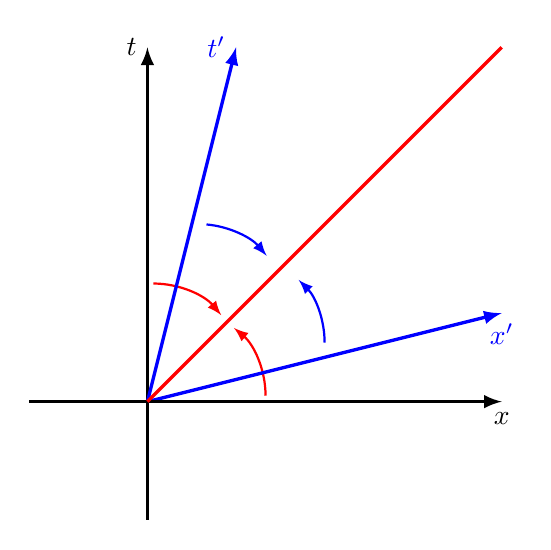
\begin{tikzpicture}[scale=0.75,>=latex]
	% Draw the time axis (t-axis)
	\draw[very thick,->] (0,-2) -- (0,6) node[left] {$t$};
	%\draw[->, thick, red] (0.1,2) arc[start angle=120, end angle=55, radius=1.5cm];
	\draw[->, thick, red] (0.1,2) arc[start angle=90, end angle=40, radius=1.5cm];
	\draw[->, thick, red] (2,0.1) arc[start angle=0, end angle=50, radius=1.5cm];
	% Draw first mover
	\draw[very thick,->, blue] (0,0) -- (1.5,6) node[left] {$t'$};
	\draw[very thick,->, blue] (0,0) -- (6,1.5) node[below] {$x'$};
	
	\draw[->, thick, blue] (3,1) arc[start angle=0, end angle=45, radius=1.5cm];
	\draw[->, thick, blue] (1,3) arc[start angle=85, end angle=40, radius=1.5cm];
	
	% Draw the space axis (x-axis)
	\draw[very thick,->] (-2,0) -- (6,0) node[below] {$x$};
	
	% Draw light
	\draw[very thick,-, red] (0,0) -- (6,6) node[left] {$ $};
	
\end{tikzpicture}

%
%%
%%% Figure 8 %%%
%%
%
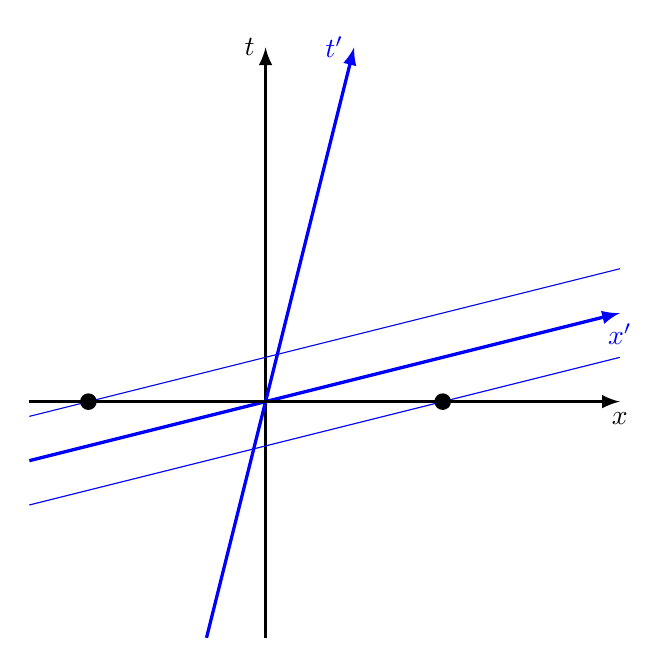
\begin{tikzpicture}[scale=0.75,>=latex]
	
	% Draw the time axis (t-axis)
	\draw[very thick,->] (0,-4) -- (0,6) node[left] {$t$};
	%\draw[->, thick, red] (0.1,2) arc[start angle=120, end angle=55, radius=1.5cm];

	% Draw first mover
	\draw[very thick,->, blue] (-1,-4) -- (1.5,6) node[left] {$t'$};
	\draw[very thick,->, blue] (-4,-1) -- (6,1.5) node[below] {$x'$};
	% y = ax + b
	% -1 = -4a + b
	% 1.5 = 6a + b
	% 2.5 = 10a a = 0.25 b = 0


	% Draw lines of simultaneity for the moving observer through the two events
	\draw[thin,-,blue] (-4,-0.25) -- (6,2.25);
	\draw[thin,-,blue] (-4,-1.75) -- (6,0.75);
	
	
	% Draw the space axis (x-axis)
	\draw[very thick,->] (-4,0) -- (6,0) node[below] {$x$};

	\fill[black] (-3,0) circle[radius=4pt];
	\fill[black] (3,0) circle[radius=4pt];
	
\end{tikzpicture}

%
%%
%%% Figure 9 %%%
%%
%
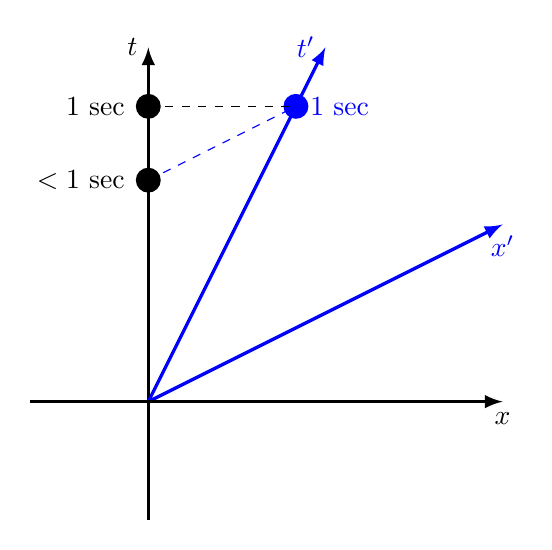
\begin{tikzpicture}[scale=0.75,>=latex]
	
	% Draw the time axis (t-axis)
	\draw[very thick,->] (0,-2) -- (0,6) node[left] {$t$};

	% Draw first mover
	\draw[very thick,->, blue] (0,0) -- (3,6) node[left] {$t'$};
	\draw[very thick,->, blue] (0,0) -- (6,3) node[below] {$x'$};
	
	% Draw the space axis (x-axis)
	\draw[very thick,->] (-2,0) -- (6,0) node[below] {$x$};

	% Draw the clock tick for moving observer and add a node label saying 1
	\fill[blue] (2.5,5) circle[radius=6pt] node[right] {$\,1$ sec};

	% Draw simultaneity line for moving clock tick
	\draw[thin,dashed,-,blue] (0,3.75) -- (2.5,5);

	% clock tick on stationary observer according to stationary observer
	\fill[black] (0,5) circle[radius=6pt] node[left] {$\,1$ sec $\,$};

	% Simultaneity line for stationary clock tick
	\draw[thin,dashed,-] (0,5) -- (2.5,5);

	% Draw clock tick for stationary observer according to moving observer
	\fill[black] (0,3.75) circle[radius=6pt] node[left] {$< 1$ sec $\,$};

\end{tikzpicture}

%%% FIGURE 10

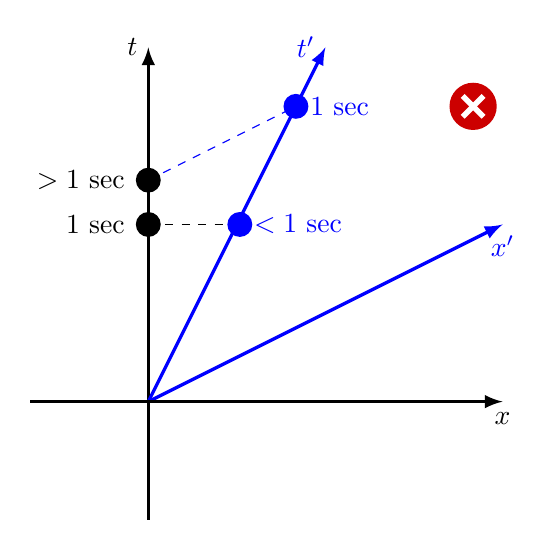
\begin{tikzpicture}[scale=0.75,>=latex]
	
	% Draw the time axis (t-axis)
	\draw[very thick,->] (0,-2) -- (0,6) node[left] {$t$};

	% Draw first mover
	\draw[very thick,->, blue] (0,0) -- (3,6) node[left] {$t'$};
	\draw[very thick,->, blue] (0,0) -- (6,3) node[below] {$x'$};
	
	% Draw the space axis (x-axis)
	\draw[very thick,->] (-2,0) -- (6,0) node[below] {$x$};

	% Draw the clock tick for moving observer and add a node label saying 1
	\fill[blue] (2.5,5) circle[radius=6pt] node[right] {$\,1$ sec};

	% Draw simultaneity line for moving clock tick
	\draw[thin,dashed,-,blue] (0,3.75) -- (2.5,5);

	% Draw clock tick for stationary observer according to moving observer
	\fill[black] (0,3.75) circle[radius=6pt] node[left] {$> 1$ sec $\,$};

	% Draw a clock tick of 1 second for stationary observer
	\fill[black] (0,3) circle[radius=6pt] node[left] {$\,1$ sec $\,$};

	% Draw black simultaneity line
	\draw[thin,dashed,-,black] (0,3) -- (1.75,3);

	% Draw blue clock tick for moving observer according to stationary observer
	\fill[blue] (1.55,3) circle[radius=6pt] node[right] {$\,<1$ sec};

	% Draw red circle with white tilted cross (danger symbol)
\begin{scope}
    \coordinate (danger) at (5.5,5); % <-- adjust position as desired
    % red circle
    \fill[red!80!black] (danger) circle[radius=0.4];
    % white cross (two lines tilted 45 degrees)
    \draw[line width=2pt, white, rotate around={45:(danger)}]
        ($(danger)+(-0.25,0)$) -- ($(danger)+(0.25,0)$);
    \draw[line width=2pt, white, rotate around={45:(danger)}]
        ($(danger)+(0,-0.25)$) -- ($(danger)+(0,0.25)$);
\end{scope}

\end{tikzpicture}

%%% FIGURE 11
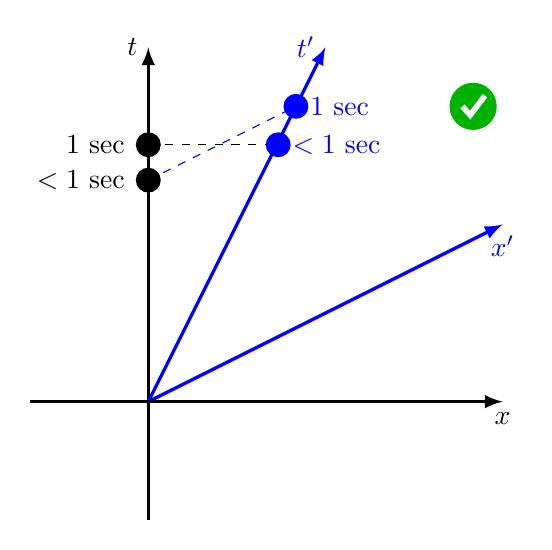
\begin{tikzpicture}[scale=0.75,>=latex]
	
		% Draw the time axis (t-axis)
	\draw[very thick,->] (0,-2) -- (0,6) node[left] {$t$};

	% Draw first mover
	\draw[very thick,->, blue] (0,0) -- (3,6) node[left] {$t'$};
	\draw[very thick,->, blue] (0,0) -- (6,3) node[below] {$x'$};
	
	% Draw the space axis (x-axis)
	\draw[very thick,->] (-2,0) -- (6,0) node[below] {$x$};

	% Draw the clock tick for moving observer and add a node label saying 1
	\fill[blue] (2.5,5) circle[radius=6pt] node[right] {$\,1$ sec};

	% Draw simultaneity line for moving clock tick
	\draw[thin,dashed,-,blue] (0,3.75) -- (2.5,5);

	% Draw clock tick for stationary observer according to moving observer
	\fill[black] (0,3.75) circle[radius=6pt] node[left] {$<1$ sec $\,$};

	% Draw a clock tick of 1 second for stationary observer
	\fill[black] (0,4.35) circle[radius=6pt] node[left] {$\,1$ sec $\,$};

	% Draw black simultaneity line
	\draw[thin,dashed,-,black] (0,4.35) -- (2.3,4.35);

	% Draw blue clock tick for moving observer according to stationary observer
	\fill[blue] (2.2,4.35) circle[radius=6pt] node[right] {$\,<1$ sec};
% Draw green circle with white checkmark (safe symbol)
\begin{scope}
    \coordinate (safe) at (5.5,5); % <-- adjust position as desired
    % green circle
    \fill[green!70!black] (safe) circle[radius=0.4];
    % white checkmark
    \draw[line width=2pt, white]
        ($(safe)+(-0.18,0.0)$) -- ($(safe)+(-0.05,-0.15)$) -- ($(safe)+(0.2,0.18)$);
\end{scope}

	
\end{tikzpicture}

%%% FIGURE 12
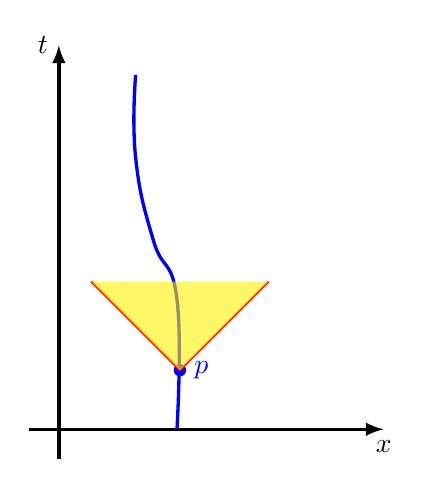
\begin{tikzpicture}[scale=0.75,>=latex]
		
		% Axes
		\draw[very thick,->] (0,-0.5) -- (0,6.5) node[left] {$t$};
		\draw[very thick,->] (-0.5,0) -- (5.5,0) node[below] {$x$};
		
		% Worldline: up (in time), then up-left, then up
		% Smooth worldline (no kinks)
		\draw[very thick,blue]
		plot [smooth, tension=0.8]
		coordinates {
			(2,0)
			(2,2.2)
			(1.6,3.2)
			(1.3,4.6)
			(1.3,6.0)
		};
		
		% Emission event on the worldline
		\coordinate (E1) at (2.05,1);
		\fill[blue] (E1) circle[radius=3pt] node[right] {$\,p$};
		
		% A small "future" light cone macro (opening at 45 degrees)
		\newcommand{\lightcone}[3]{% apex (#1), height #2, half-width #3
			\draw[thick,red] (#1) -- ++(#3,#2);
			\draw[thick,red] (#1) -- ++(-#3,#2);
			\fill[yellow,opacity=0.6] (#1) -- ++(#3,#2) -- ++(-2*#3,0) -- cycle;
		}
		
		\lightcone{E1}{1.5}{1.5}
	\end{tikzpicture}


%%% FIGURE 13
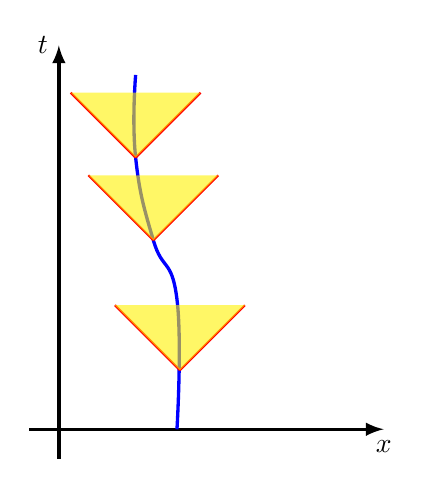
\begin{tikzpicture}[scale=0.75,>=latex]
		
		% Axes
		\draw[very thick,->] (0,-0.5) -- (0,6.5) node[left] {$t$};
		\draw[very thick,->] (-0.5,0) -- (5.5,0) node[below] {$x$};
		
		% Worldline: up (in time), then up-left, then up
		% Smooth worldline (no kinks)
		\draw[very thick,blue]
		plot [smooth, tension=0.8]
		coordinates {
			(2,0)
			(2,2.2)
			(1.6,3.2)
			(1.3,4.6)
			(1.3,6.0)
		};
		
		% Mark the three emission events on the worldline
		\coordinate (E1) at (2.05,1);
		\coordinate (E2) at (1.6,3.2);
		\coordinate (E3) at (1.3,4.6);

		% A small "future" light cone macro (opening at 45 degrees)
		\newcommand{\lightcone}[3]{% apex (#1), height #2, half-width #3
			\draw[thick,red] (#1) -- ++(#3,#2);
			\draw[thick,red] (#1) -- ++(-#3,#2);
			\fill[yellow,opacity=0.6] (#1) -- ++(#3,#2) -- ++(-2*#3,0) -- cycle;
		}
		
		% Draw three small cones starting at those points
		\lightcone{E1}{1.1}{1.1}
		\lightcone{E2}{1.1}{1.1}
		\lightcone{E3}{1.1}{1.1}
		
	\end{tikzpicture}

%%% FIGURE 14
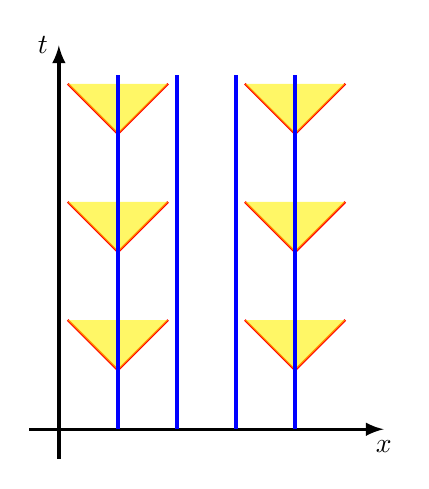
\begin{tikzpicture}[scale=0.75,>=latex]

% Draw the time axis (t-axis)
\draw[very thick,->] (0,-0.5) -- (0,6.5) node[left] {$t$};

% A small "future" light cone macro (opening at 45 degrees)
\newcommand{\lightcone}[3]{% apex (#1), height #2, half-width #3
	\draw[thick,red] (#1) -- ++(#3,#2);
	\draw[thick,red] (#1) -- ++(-#3,#2);
	\fill[yellow,opacity=0.6] (#1) -- ++(#3,#2) -- ++(-2*#3,0) -- cycle;
}

\coordinate (E1) at (1,1);
\coordinate (E2) at (1,3);
\coordinate (E3) at (1,5);
\coordinate (E4) at (4,1);
\coordinate (E5) at (4,3);
\coordinate (E6) at (4,5);

\lightcone{E1}{0.85}{0.85}
\lightcone{E2}{0.85}{0.85}
\lightcone{E3}{0.85}{0.85}
\lightcone{E4}{0.85}{0.85}
\lightcone{E5}{0.85}{0.85}
\lightcone{E6}{0.85}{0.85}

% Draw the space axis (x-axis)
\draw[very thick,->] (-0.5,0) -- (5.5,0) node[below] {$x$};

\foreach \x in {1,2,3,4}
\draw[very thick, blue] (\x,0) -- (\x, 6);
\end{tikzpicture}

%%% FIGURE 15
\begin{tikzpicture}	
\begin{axis}[
	set layers,
	axis on top,
    width=8cm, height=8cm,
    axis lines=middle,
	axis line style={thick},
	grid=both,
	grid style={line width=.1pt, draw=gray!10},
    xlabel={$r$},
	xlabel style={
    	at={(axis description cs:1,0)},
    	anchor=west},
	ylabel={$t$},
	ylabel style={
    	at={(axis description cs:0,1)},
    	anchor=south},
    xmin= 0, xmax=100,   % set to match python numerics
    ymin= 0, ymax=100,   % set to match python numerics
    xtick=\empty,
	ytick=\empty,
	clip = true
]

\pgfmathsetmacro{\rs}{10} % Schwarzschild radius same as in python numerics
\pgfmathsetmacro{\bodyedge}{20} % Where to start shading the central body

\begin{pgfonlayer}{axis background}
	% Plot N trajectories
	\foreach \i in {1,...,5} { % <-- set 6 = N
	 \addplot[very thick, blue] table [x=r, y=t, col sep=comma]
	 {../data_pg/traj_\i.csv};
	}
\end{pgfonlayer}

\begin{pgfonlayer}{axis foreground}
	% Horizon shading
	\addplot[name path=left, draw=none] coordinates {(0.05,0) (0.05,100)};
	\addplot[name path=right, draw=none] coordinates {(\bodyedge,0) (\bodyedge,100)};
	\addplot[fill=black!15, draw=none] fill between[of=left and right];
\end{pgfonlayer}

\end{axis}
\end{tikzpicture}

%%% Figure 16
\begin{tikzpicture}	
\begin{axis}[
	set layers,
	axis on top,
    width=8cm, height=8cm,
    axis lines=middle,
	axis line style={thick},
	grid=both,
	grid style={line width=.1pt, draw=gray!10},
    xlabel={$r$},
	xlabel style={
    	at={(axis description cs:1,0)},
    	anchor=west},
	ylabel={$t$},
	ylabel style={
    	at={(axis description cs:0,1)},
    	anchor=south},
    xmin= 0, xmax=100,   % set to match your figure
    ymin= 0, ymax=100,   % set to match your figure
    xtick=\empty,
	ytick=\empty,
	clip = true,	
]

\pgfmathsetmacro{\rs}{10} % Schwarzschild radius (must be consistent with python numerics)
\pgfmathsetmacro{\bodyedge}{20} % where to start shading the central body (must be > \rs)

\begin{pgfonlayer}{axis background}
% Plot N trajectories
\foreach \i in {1,...,5} { % <-- set 6 = N
 \addplot[very thick, blue] table [x=r, y=t, col sep=comma]
 {../data_pg/traj_\i.csv};
}


%Plot the lightcones at calculated locations
\csvreader[
  separator=comma
]{../data_pg/cone_points.csv}{}{% no column names
  \lightconecurved{\csvcoli}{\csvcolii}{10}{\csvcoliv}{\rs}%
}
\end{pgfonlayer}

\begin{pgfonlayer}{axis foreground}
% Horizon shading
\addplot[name path=left, draw=none] coordinates {(0.05,0) (0.05,100)};
\addplot[name path=right, draw=none] coordinates {(\bodyedge,0) (\bodyedge,100)};
\addplot[fill=black!15, draw=none] fill between[of=left and right];
\end{pgfonlayer}


\end{axis}
\end{tikzpicture}

%%% Figure 17
\begin{tikzpicture}	
\begin{axis}[
	set layers,
	axis on top,
    width=8cm, height=8cm,
    axis lines=middle,
	axis line style={thick},
	grid=both,
	grid style={line width=.1pt, draw=gray!10},
    xlabel={$r$},
	xlabel style={
    	at={(axis description cs:1,0)},
    	anchor=west},
	ylabel={$t$},
	ylabel style={
    	at={(axis description cs:0,1)},
    	anchor=south},
    xmin= 0, xmax=100,   % set to match your figure
    ymin= 0, ymax=100,   % set to match your figure
    xtick=\empty,
	ytick=\empty,
	clip = true,	
]

\pgfmathsetmacro{\rs}{25} % Schwarzschild radius (must be consistent with python numerics)
\pgfmathsetmacro{\bodyedge}{25} % where to start shading the central body

% Horzion line
\addplot[thin, dashed] coordinates {(\rs,0) (\rs,100)};

% Plot N trajectories
\foreach \i in {1,...,5} { % <-- set  = N
 \addplot[very thick, blue] table [x=r, y=t, col sep=comma]
 {../data_pg/traj_bh_\i.csv};
}

% Plot the lightcones at calculated locations
\csvreader[
  separator=comma
]{../data_pg/cone_points_bh.csv}{}{% no column names
  \lightconecurved{\csvcoli}{\csvcolii}{10}{\csvcoliv}{\rs}%
}
\end{axis}
\end{tikzpicture}


\end{document}